
%(BEGIN_QUESTION)
% Copyright 2011, Tony R. Kuphaldt, released under the Creative Commons Attribution License (v 1.0)
% This means you may do almost anything with this work of mine, so long as you give me proper credit

Many flammable gases are produced in chemical processing and oil refineries as ``waste'' products.  These ``waste'' gases may be used as fuel for steam boilers and combustion heaters in other parts of the refinery.  The problem is, ``waste'' fuel gas production is often unsteady, and the demand for fuel gas in boilers and heaters is unsteady as well.  There are times when there will be a surplus of waste gas (more than can be used), and times when there will not be enough.

The following pressure control system works to maintain constant fuel gas pressure in the accumulator vessel despite changes in waste gas flows and fuel gas demands:

$$\includegraphics[width=15.5cm]{i00077x01.eps}$$

Control valves PV-45a and PV-45b are split-ranged, electrically connected in series to operate off the same 4-20 mA signal from PIC-45.  The controller itself is direct-acting, and the valves' split-range calibrations are as follows:

% No blank lines allowed between lines of an \halign structure!
% I use comments (%) instead, so that TeX doesn't choke.

$$\vbox{\offinterlineskip
\halign{\strut
\vrule \quad\hfil # \ \hfil & 
\vrule \quad\hfil # \ \hfil & 
\vrule \quad\hfil # \ \hfil \vrule \cr
\noalign{\hrule}
%
% First row
{\bf Valve} & {\bf Fully closed at} & {\bf Fully open at} \cr
%
\noalign{\hrule}
%
% Another row
PV-45a & 12 mA & 4 mA \cr
%
\noalign{\hrule}
%
% Another row
PV-45b & 12 mA & 20 mA \cr
%
\noalign{\hrule}
} % End of \halign 
}$$ % End of \vbox

An operator happens to notice a low pressure indication registered on PI-44: 23 PSI.  The controller setpoint is 30 PSI, and the operator calls the control room on her radio to verify the setpoint is still at 30 PSI.  Worried, she then calls you over to investigate the problem with her.  Your first diagnostic test is to call the control operator on your radio and ask what the pressure indication reads for PIC-45.  The control room operator calls back to tell you PIC-45 reads 22.8 PSI.

\vskip 10pt

Explain how you would proceed troubleshooting this problem.  What are some likely causes for the low pressure, and what would your next diagnostic step(s) be?  Do you think PSV-14 could be at fault?  If your next step was to take an electrical measurement somewhere in the signal wiring of this system, what measurement would you take and what might that measurement tell you about the nature of the problem?

\underbar{file i00077}
%(END_QUESTION)





%(BEGIN_ANSWER)

There is reason to believe the low pressure is real, because the two pressure readings agree with each other.  This means the problem -- whatever it is -- is not in the transmitter (PT-45) or in the controller input, but is most likely in the final control element side of the loop.

PSV-14 is a pressure safety valve providing over-pressure protection for the accumulator vessel, but it is unlikely to be the source of trouble.  If PSV-14 were ``lifting'' when it should not be (at this low of pressure!), the noise it would be making would be quite substantial and likely to attract the attention of the field operator who knows well what the process should sound like.

%(END_ANSWER)





%(BEGIN_NOTES)

The problem could be PV-45a failing to open as far as it should, or PV-45b passing flow when it should not be passing flow.  A quick measurement of PIC-45's output 4-20 mA signal would be a good diagnostic measurement to take, combined with an observation of the stem positions for PV-45a and PV-45b.  Either one (or more?) of the control valves is not responding the way it should, or the controller is not responding the way it should to the low pressure.  The controller's output signal {\it should} be high (20 mA?) as it senses a low process variable (22.8 PSI) compared to its setpoint of 30 PSI.








\filbreak \vskip 20pt \vbox{\hrule \hbox{\strut \vrule{} {\bf Virtual Troubleshooting} \vrule} \hrule}

\noindent
{\bf Predicting the effect of a given fault:} present each of the following faults to the students, one at a time, having them comment on all the effects each fault would produce.

\begin{itemize}
\item{} 
\item{} 
\item{} 
\end{itemize}


\vskip 10pt


\noindent
{\bf Identifying possible/impossible faults:} present symptoms to the students and then have them determine whether or not a series of suggested faults could account for all the symptoms, explaining {\it why} or {\it why not} for each proposed fault:

\begin{itemize}
\item{} Symptom: {\it Accumulator pressure is 47 PSI when controller setpoint is 30 PSI}
\item{} PV-45a valve air supply failed
\item{} PV-45b valve air supply failed
\item{} Open signal cable at controller output
\item{} Shorted signal cable at controller output
\item{} Open signal cable at controller PV input
\item{} Shorted signal cable at controller PV input
\item{} Burner fuel gas line block valve shut
\item{} Flare line block valve shut
\end{itemize}


\vskip 10pt


\noindent
{\bf Determining the utility of given diagnostic tests:} present symptoms to the students and then propose the following diagnostic tests one by one.  Students rate the value of each test, determining whether or not it would give useful information (i.e. tell us something we don't already know).  Students determine what different results for each test would indicate about the fault, if anything:

\begin{itemize}
\item{} Symptom: {\it }
\item{}  -- {\bf Yes/No}
\item{}  -- {\bf Yes/No}
\end{itemize}


\vskip 10pt


\noindent
{\bf Diagnosing a fault based on given symptoms:} imagine the ??? fails ??? in this system (don't reveal the fault to students!).  Present the operator's observation(s) to the students, have them consider possible faults and diagnostic strategies, and then tell them the results of tests they propose based on the following symptoms, until they have properly identified the nature and location of the fault:

\begin{itemize}
\item{} {\it }
\item{} 
\item{} 
\end{itemize}


%INDEX% Basics, control loop troubleshooting: determining cause of control problem
%INDEX% Final Control Elements, valve: split-ranging

%(END_NOTES)


